\documentclass[../../main.tex]{subfiles}

\begin{document}

This view describes the behavior and interaction of the system’s building blocks as runtime elements.

\newcounter{RuntimeScenarioCounter}

\stepcounter{RuntimeScenarioCounter}
\subsection{Runtime Scenario \arabic{RuntimeScenarioCounter} - Store employees login}

\begin{figure}[H]
    \centering
    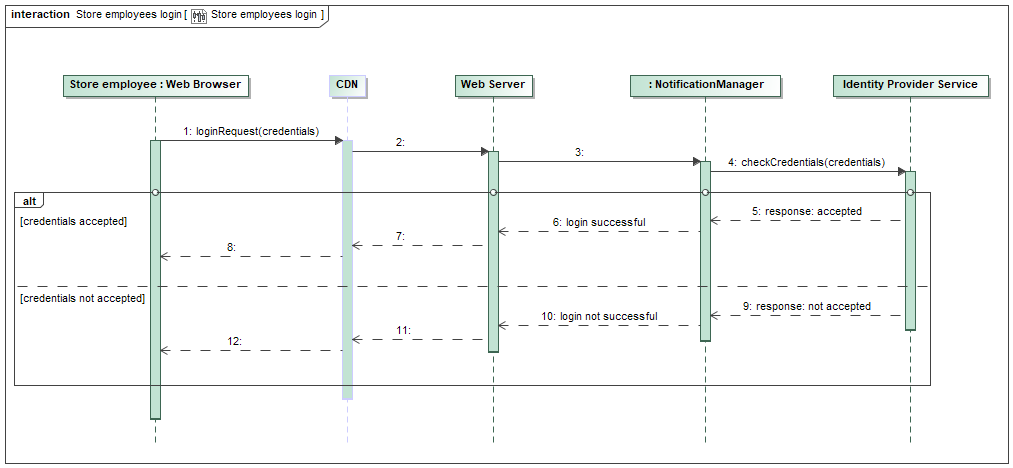
\includegraphics[width=\textwidth]{Store_employees_login.png}
    \caption{
        Store employees login sequence diagram.
    }
\end{figure}

\stepcounter{RuntimeScenarioCounter}
\subsection{Runtime Scenario \arabic{RuntimeScenarioCounter} - Definition of safety standard parameters}
% store manager already logged in
\begin{figure}[H]
    \centering
    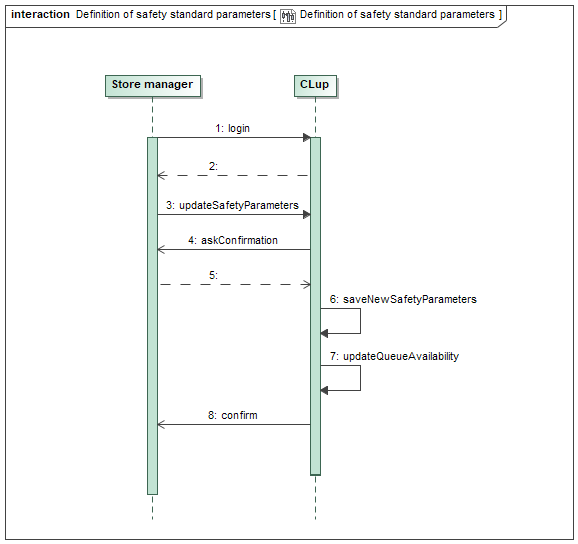
\includegraphics[width=\textwidth]{Definition_of_safety_standard_parameters.png}
    \caption{
        Definition of safety standard parameters sequence diagram.
    }
\end{figure}


\stepcounter{RuntimeScenarioCounter}
\subsection{Runtime Scenario \arabic{RuntimeScenarioCounter} - Consulting statistics}
% store manager already logged in
\begin{figure}[H]
    \centering
    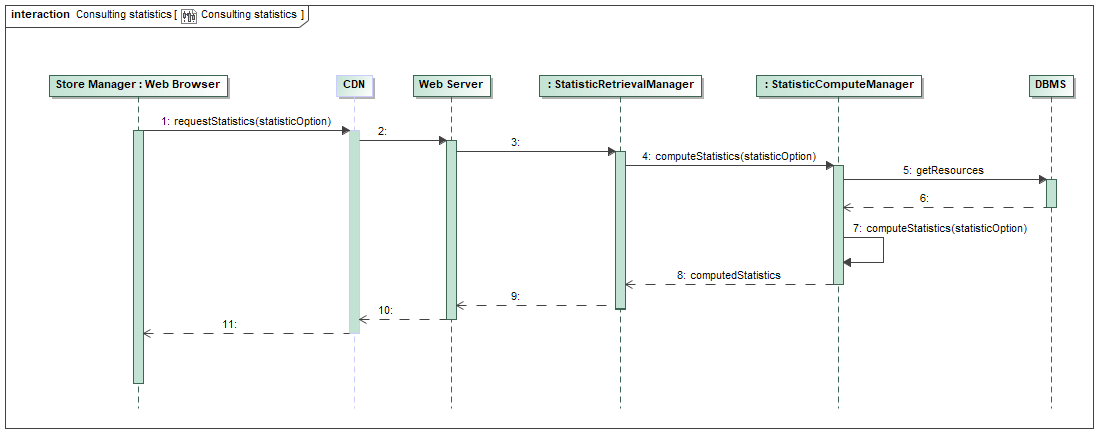
\includegraphics[width=\textwidth]{Consulting_statistics.png}
    \caption{
        Consulting statistics sequence diagram.
    }
\end{figure}


\stepcounter{RuntimeScenarioCounter}
\subsection{Runtime Scenario \arabic{RuntimeScenarioCounter} - In presence ticket generation}
% another for numeric code
% store employee already logged in
\begin{figure}[H]
    \centering
    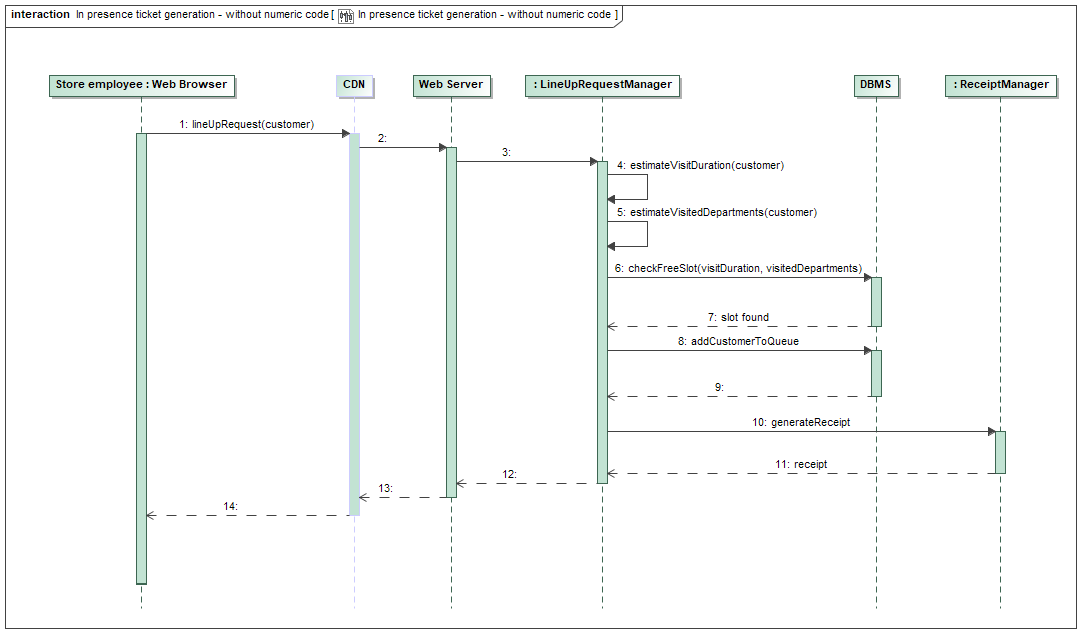
\includegraphics[width=\textwidth]{In_presence_ticket_generation_-_without_numeric_code.png}
    \caption{
        In presence ticket generation - without numeric code sequence diagram.
    }
\end{figure}

\begin{figure}[H]
    \centering
    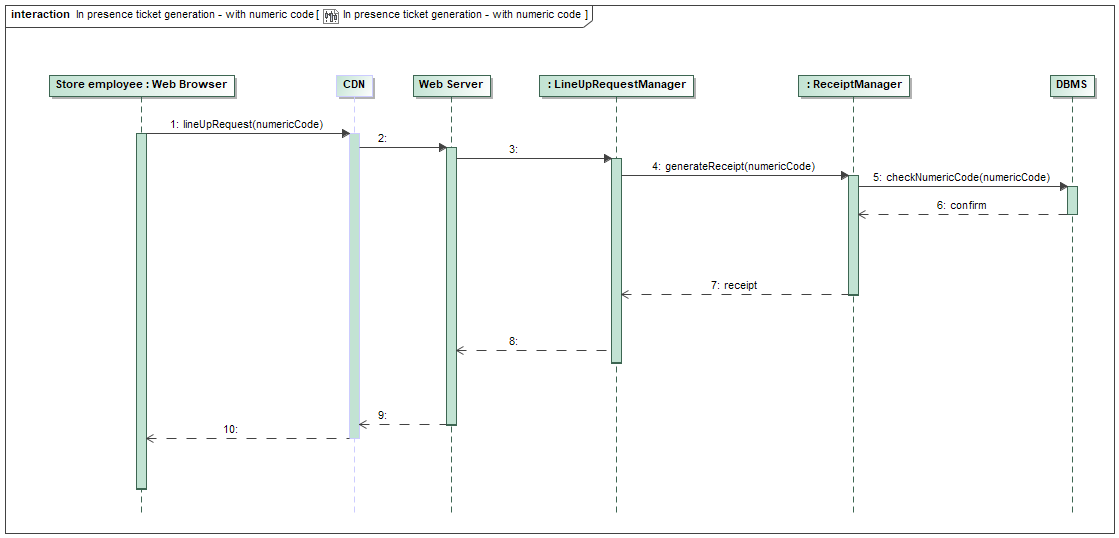
\includegraphics[width=\textwidth]{In_presence_ticket_generation_-_with_numeric_code.png}
    \caption{
        In presence ticket generation - with numeric code sequence diagram.
    }
\end{figure}

\stepcounter{RuntimeScenarioCounter}
\subsection{Runtime Scenario \arabic{RuntimeScenarioCounter} - Immediate queueing with telephone}
% Could this be general for both telephone and IT device? NO

\begin{figure}[H]
    \centering
    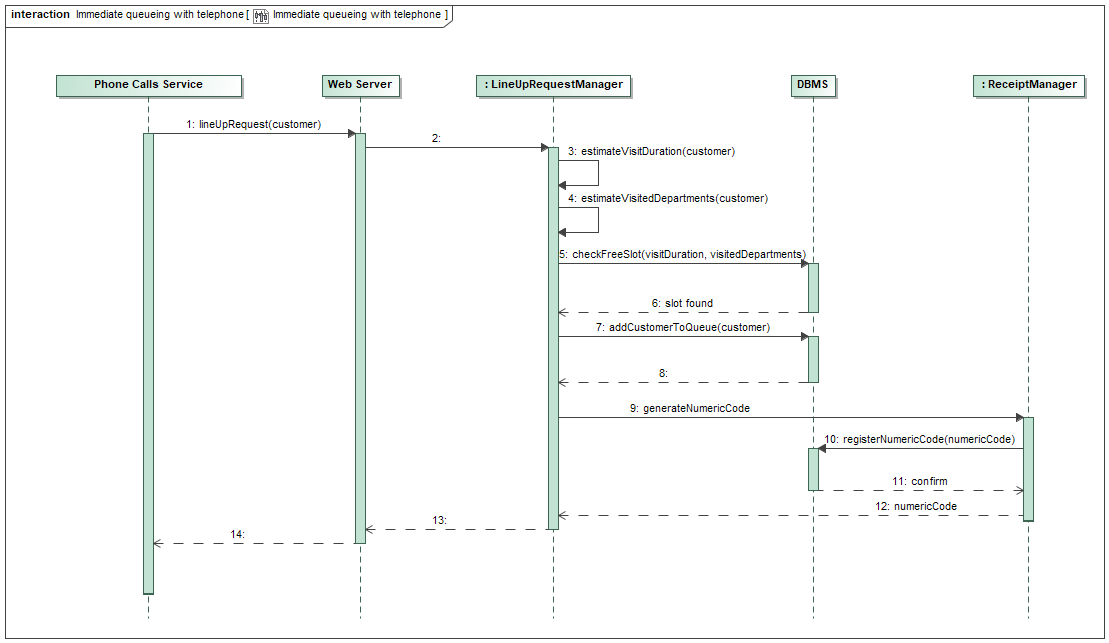
\includegraphics[width=\textwidth]{Immediate_queueing_with_telephone.png}
    \caption{
        Immediate queueing with telephone sequence diagram.
    }
\end{figure}

\stepcounter{RuntimeScenarioCounter}
\subsection{Runtime Scenario \arabic{RuntimeScenarioCounter} - Reservation}
% Could this be general for both telephone and IT device? NO

\begin{figure}[H]
    \centering
    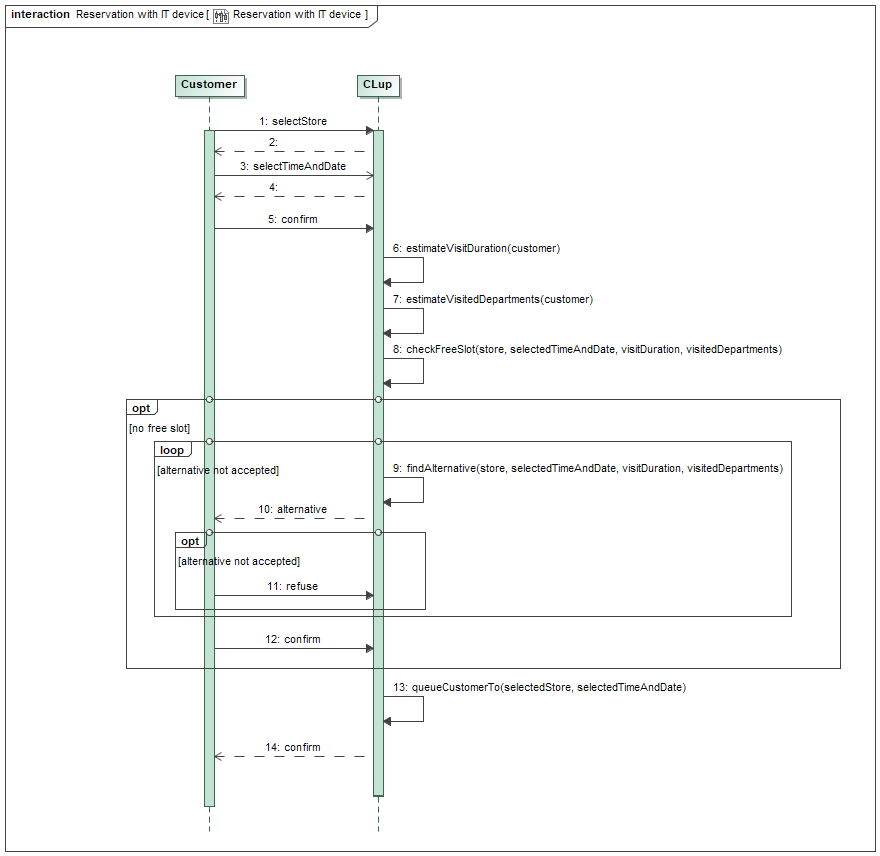
\includegraphics[width=\textwidth]{Reservation_with_IT_device.png}
    \caption{
        Reservation with IT device sequence diagram.
    }
\end{figure}

\begin{figure}[H]
    \centering
    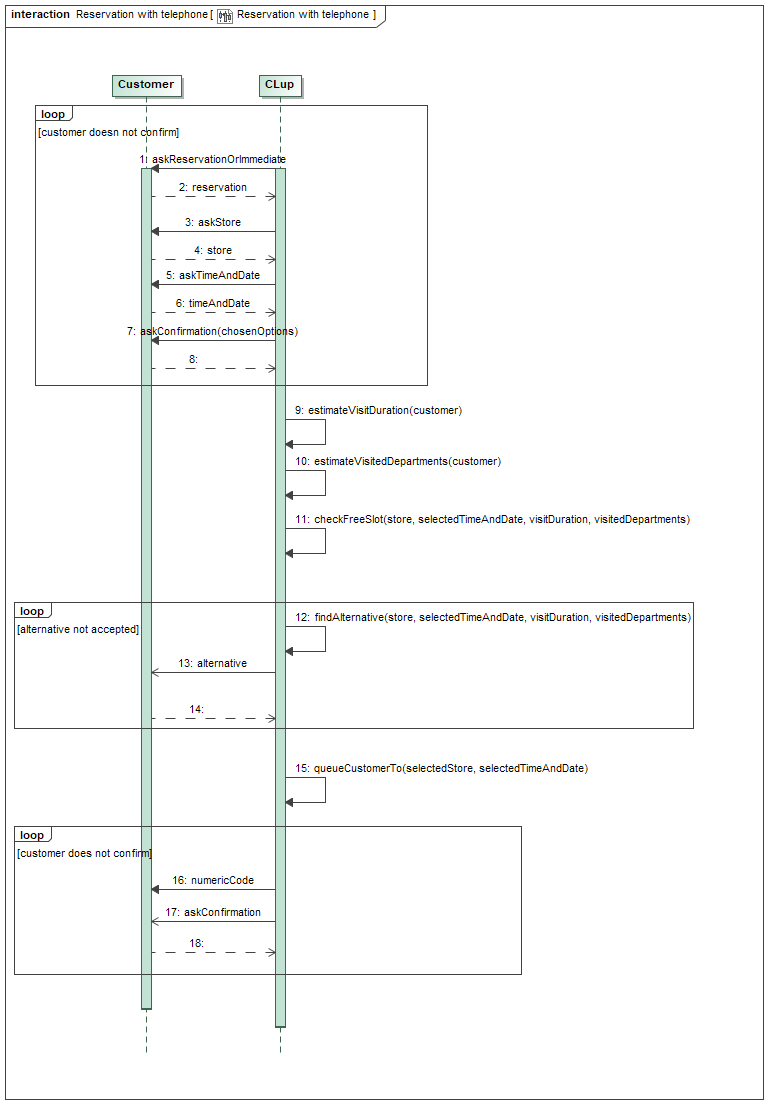
\includegraphics[width=\textwidth]{Reservation_with_telephone.png}
    \caption{
        Reservation with telephone sequence diagram.
    }
\end{figure}

\stepcounter{RuntimeScenarioCounter}
\subsection{Runtime Scenario \arabic{RuntimeScenarioCounter} - Cancellation}

\begin{figure}[H]
    \centering
    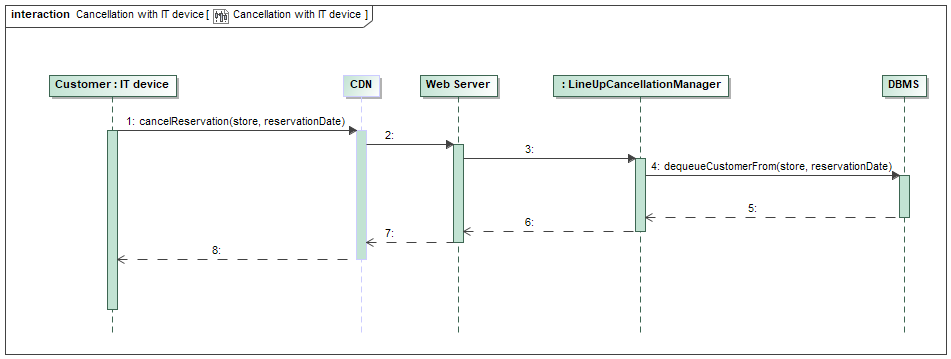
\includegraphics[width=\textwidth]{Cancellation_with_IT_device.png}
    \caption{
        Cancellation with IT device sequence diagram.
    }
\end{figure}

\begin{figure}[H]
    \centering
    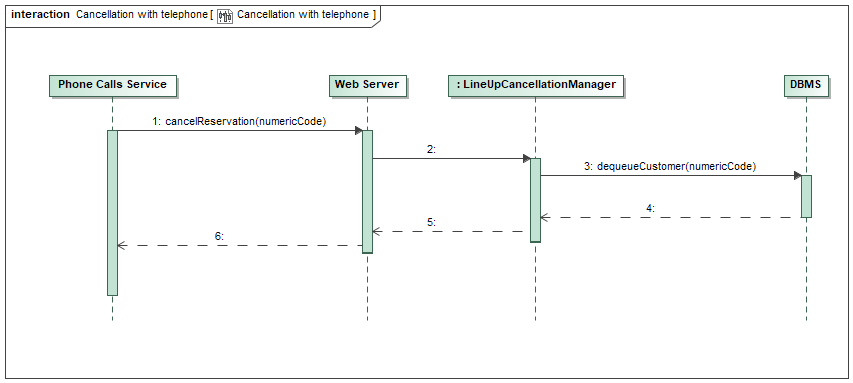
\includegraphics[width=\textwidth]{Cancellation_with_telephone.png}
    \caption{
        Cancellation with telephone sequence diagram.
    }
\end{figure}

\stepcounter{RuntimeScenarioCounter}
\subsection{Runtime Scenario \arabic{RuntimeScenarioCounter} - CLup notification}
% do both IT and telephone

\begin{figure}[H]
    \centering
    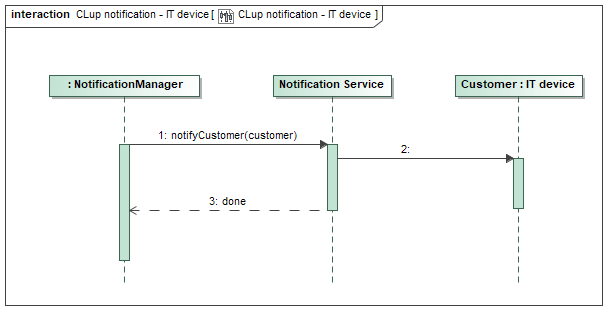
\includegraphics[width=\textwidth]{CLup_notification_-_IT_device.png}
    \caption{
        CLup notification - IT device sequence diagram.
    }
\end{figure}

\begin{figure}[H]
    \centering
    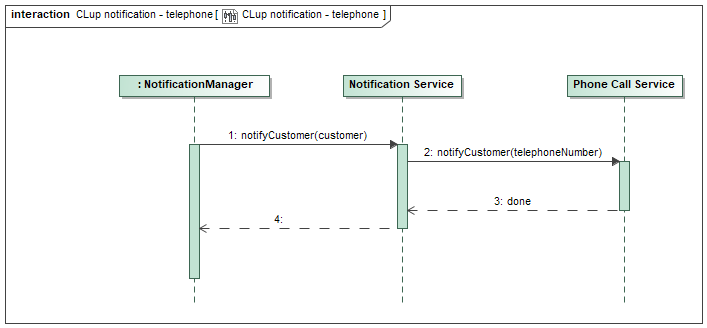
\includegraphics[width=\textwidth]{CLup_notification_-_telephone.png}
    \caption{
        CLup notification - telephone sequence diagram.
    }
\end{figure}

\stepcounter{RuntimeScenarioCounter}
\subsection{Runtime Scenario \arabic{RuntimeScenarioCounter} - Store access}

\begin{figure}[H]
    \centering
    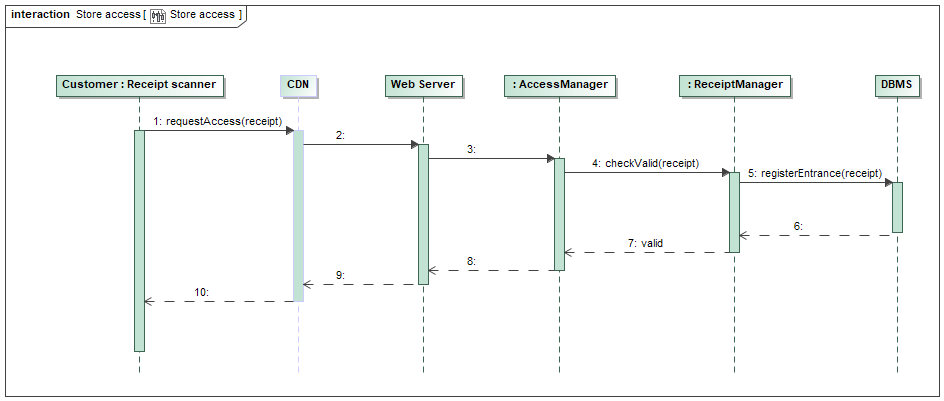
\includegraphics[width=\textwidth]{Store_access.png}
    \caption{
        Store access sequence diagram.
    }
\end{figure}

\stepcounter{RuntimeScenarioCounter}
\subsection{Runtime Scenario \arabic{RuntimeScenarioCounter} - Store exit}

\begin{figure}[H]
    \centering
    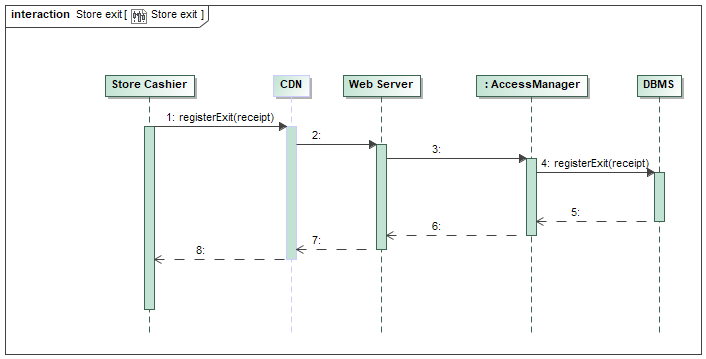
\includegraphics[width=\textwidth]{Store_exit.png}
    \caption{
        Store exit sequence diagram.
    }
\end{figure}

\end{document}


%--
% - StoresManager (per lo store manager per regolare i paramteri + per i clients per listare gli stores)
% - AuthenticationManager
% - LineUpManager (collection/package) - do not show
%   - LineUpSuggestionsManager
%   - LineUpCancellationManager
%   - LineUpRequestManager
% - NotificationManager (communicates via Notification service)
% - AccessManager
% - ReceiptManager
% - StatisticsManager (collection/package) - do not show
%   - StatisticsComputationManager
%   - StatisticsRetrievalManager
% - DBMS
% - Notification Service
% - Phone Calls service (communicates via web server)
%--
